\documentclass[12pt]{article}
\usepackage[english]{babel}
\usepackage{natbib}
\usepackage{url}
\usepackage[utf8x]{inputenc}
\usepackage{amsmath}
\usepackage{graphicx}
\graphicspath{{images/}}
\usepackage{parskip}
\usepackage{fancyhdr}
\usepackage{vmargin}
\setmarginsrb{3 cm}{2.5 cm}{3 cm}{2.5 cm}{1 cm}{1.5 cm}{1 cm}{1.5 cm}

\title{IF654 - Machine Learning}								% Title
%\author{13103057}								% Author
\date{12 Sept 2015}											% Date

\makeatletter
\let\thetitle\@title
\let\theauthor\@author
\let\thedate\@date
\makeatother

\pagestyle{fancy}
\fancyhf{}
\rhead{\theauthor}
\lhead{\thetitle}
\cfoot{\thepage}

\begin{document}

%%%%%%%%%%%%%%%%%%%%%%%%%%%%%%%%%%%%%%%%%%%%%%%%%%%%%%%%%%%%%%%%%%%%%%%%%%%%%%%%%%%%%%%%%

\begin{titlepage}
	\centering
    \vspace*{0.5 cm}
    
\includegraphics[scale = 0.1]{logo-umn.png}\\[1.0 cm]	% University Logo
    \textsc{\LARGE Machine Learning Project}\\[2.0 cm]	% University Name
	%\textsc{\Large Predicting A Pulsar Star}\\[0.5 cm]				% Course Code
	\rule{\linewidth}{0.2 mm} \\[1.5 cm]
	 \textsc{\LARGE Predicting A Pulsar Star}\\[1.0 cm]
%	{ \huge \bfseries \thetitle}\\
	\rule{\linewidth}{0.2 mm} \\[1.5 cm]
	
	\begin{minipage}{0.4\textwidth}
		\begin{flushleft} \large
		%	\emph{Submitted To:}\\
		%	Ashish Kumar\\
         %   Asst. Professor\\
          %  Computer Science Department\\
			\end{flushleft}
			\end{minipage}~
			\begin{minipage}{0.4\textwidth}
            
			\begin{flushright} \large
			\emph{Submitted By :} \\[0.5 cm]
			Steven - 13433\\
			B. Bias A. Ch. - 13536\\
			Raynaldi - 13654\\
		\end{flushright}
        
	\end{minipage}\\[2 cm]
	
	
    
    
    
    
	
\end{titlepage}

%%%%%%%%%%%%%%%%%%%%%%%%%%%%%%%%%%%%%%%%%%%%%%%%%%%%%%%%%%%%%%%%%%%%%%%%%%%%%%%%%%%%%%%%%

\tableofcontents
\pagebreak

%%%%%%%%%%%%%%%%%%%%%%%%%%%%%%%%%%%%%%%%%%%%%%%%%%%%%%%%%%%%%%%%%%%%%%%%%%%%%%%%%%%%%%%%%

\section{Identifikasi Masalah}

HTRU2 adalah kumpulan data yang menggambarkan sampel kandidat pulsar yang dikumpulkan selama Survei Alam Semesta Resolusi Tinggi. \cite{datasets}

Pulsar adalah jenis bintang Neutron yang langka yang menghasilkan emisi radio yang dapat dideteksi di Bumi. Mereka sangat menarik secara ilmiah sebagai wahana ruang-waktu, medium antar-bintang, dan keadaan materi.

Setiap pulsar menghasilkan pola emisi yang sedikit berbeda, yang sedikit berbeda pada setiap putaran. Dengan demikian deteksi sinyal potensial yang dikenal sebagai 'kandidat', dirata-ratakan pada banyak rotasi pulsar, sebagaimana ditentukan oleh panjang pengamatan. Dengan tidak adanya info tambahan, masing-masing kandidat berpotensi menggambarkan pulsar yang sebenarnya. Namun dalam praktiknya hampir semua deteksi disebabkan oleh interferensi frekuensi radio (RFI) dan kebisingan, membuat sinyal yang sah sulit ditemukan.

Alat pembelajaran mesin sekarang digunakan untuk secara otomatis melabeli kandidat pulsar untuk memfasilitasi analisis yang cepat. Sistem klasifikasi khususnya sedang banyak diadopsi, yang memperlakukan set data kandidat sebagai masalah klasifikasi biner. Di sini contoh pulsar yang sah adalah kelas positif minoritas, dan contoh palsu adalah kelas negatif mayoritas.

Kumpulan data yang dibagikan di sini berisi 16.259 contoh palsu yang disebabkan oleh RFI / noise, dan 1.639 contoh pulsar nyata. Semua contoh ini telah diperiksa oleh annotator manusia.

Setiap baris mencantumkan variabel terlebih dahulu, dan label kelas adalah entri terakhir. Label kelas yang digunakan adalah 0 (negatif) dan 1 (positif).

\hspace{1 cm}

\newpage

%%%%%%%%%%%%%%%%%%%%%%%%%%%%%%%%%%%%%%%%%%%%%%%%%%%%%%%%%%%%%%%%%%%%%%%%%%%%%%%%%%%%%%%%%

\section{Analisis Dataset}

    \subsection{Informasi Dataset}
    
    \newline Setiap kandidat dijelaskan oleh 8 variabel kontinu, dan variabel kelas tunggal. Empat yang pertama adalah statistik sederhana yang diperoleh dari profil pulsa terintegrasi (profil terlipat). Ini adalah array variabel kontinu yang menggambarkan versi sinyal bujur yang diselesaikan yang telah dirata-rata dalam waktu dan frekuensi. Empat variabel sisanya diperoleh dengan cara yang sama dari kurva DM-SNR ini dirangkum di bawah ini:
    
    \begin{enumerate}
    
        \item Mean of the integrated profile
        \newline
        Gelombang dari sebuah pulsar periodik emisi, rata-rata serentak selama beberapa ratus pulsa atau lebih. Juga dikenal sebagai profil terintegrasi.
        
        \item Standard deviation of the integrated profile.
        \item Excess kurtosis of the integrated profile.
        \item Skewness of the integrated profile.
        \newline
        Ukuran dari asimetri distribusi. Bisa nol jika distribusinya simetris, tetapi juga negatif atau positif.
        
        \item Mean of the DM-SNR curve.
        \item Standard deviation of the DM-SNR curve.
        \item Excess kurtosis of the DM-SNR curve.
        \item Skewness of the DM-SNR curve.
        \item Class.
        
    \end{enumerate}
    
    Ringkasan HTRU2 17.898 total contoh.
    \newline
    1.639 contoh positif. 16.259 contoh negatif.
    \newline
    
    \newpage
    
    \subsection{Exploratory Data Analysis}
    
    \begin{enumerate}
    
        \item Loading Dataset
        \newline 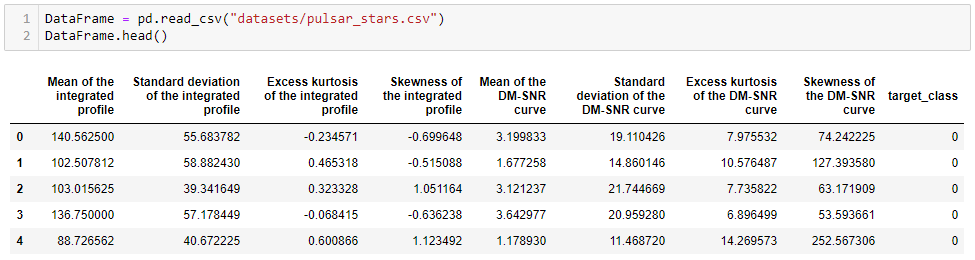
\includegraphics[scale=0.5125]{data-head.png}
        \newline
        
        \item Cek apakah ada data yang null
        \newline 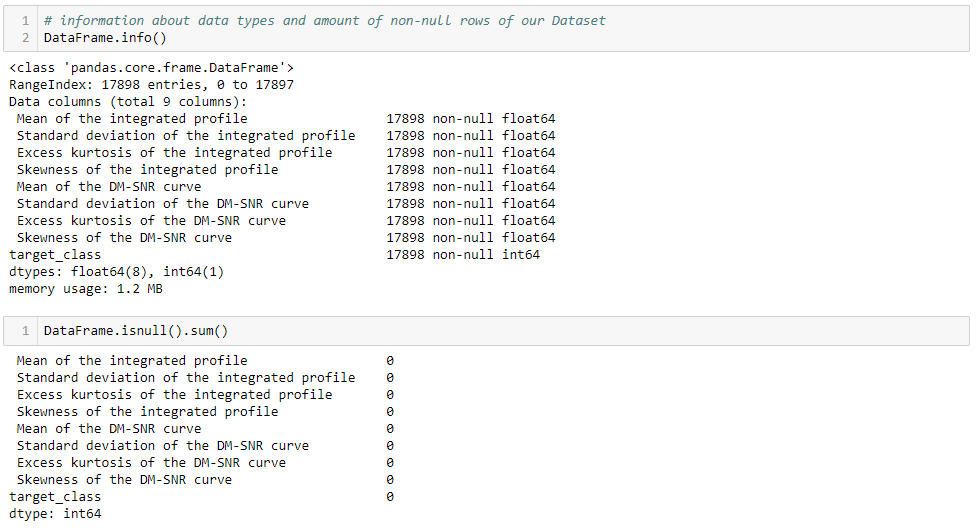
\includegraphics[scale=0.5125]{data-info.png}
        \newline Karena tidak ada data yang null, tidak diperlukan transformasi data ataupun pembersihan data.
        
        \item Lihat data statistik
        \newline 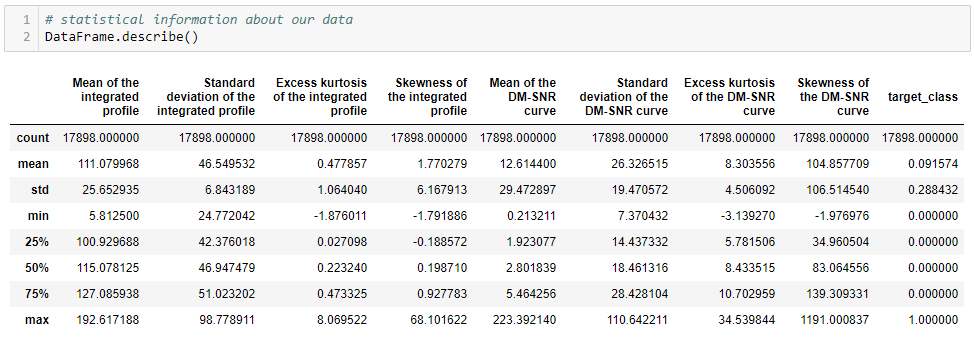
\includegraphics[scale=0.5125]{data-describe.png}
        
        \newpage
        
        \item Perbandingan porsi Target
        \newline 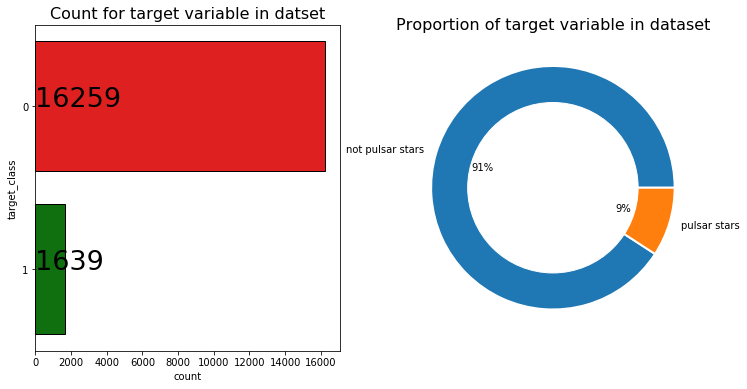
\includegraphics[scale=0.5]{proportion-target.png}
        
        \item Korelasi variabel data
        \newline 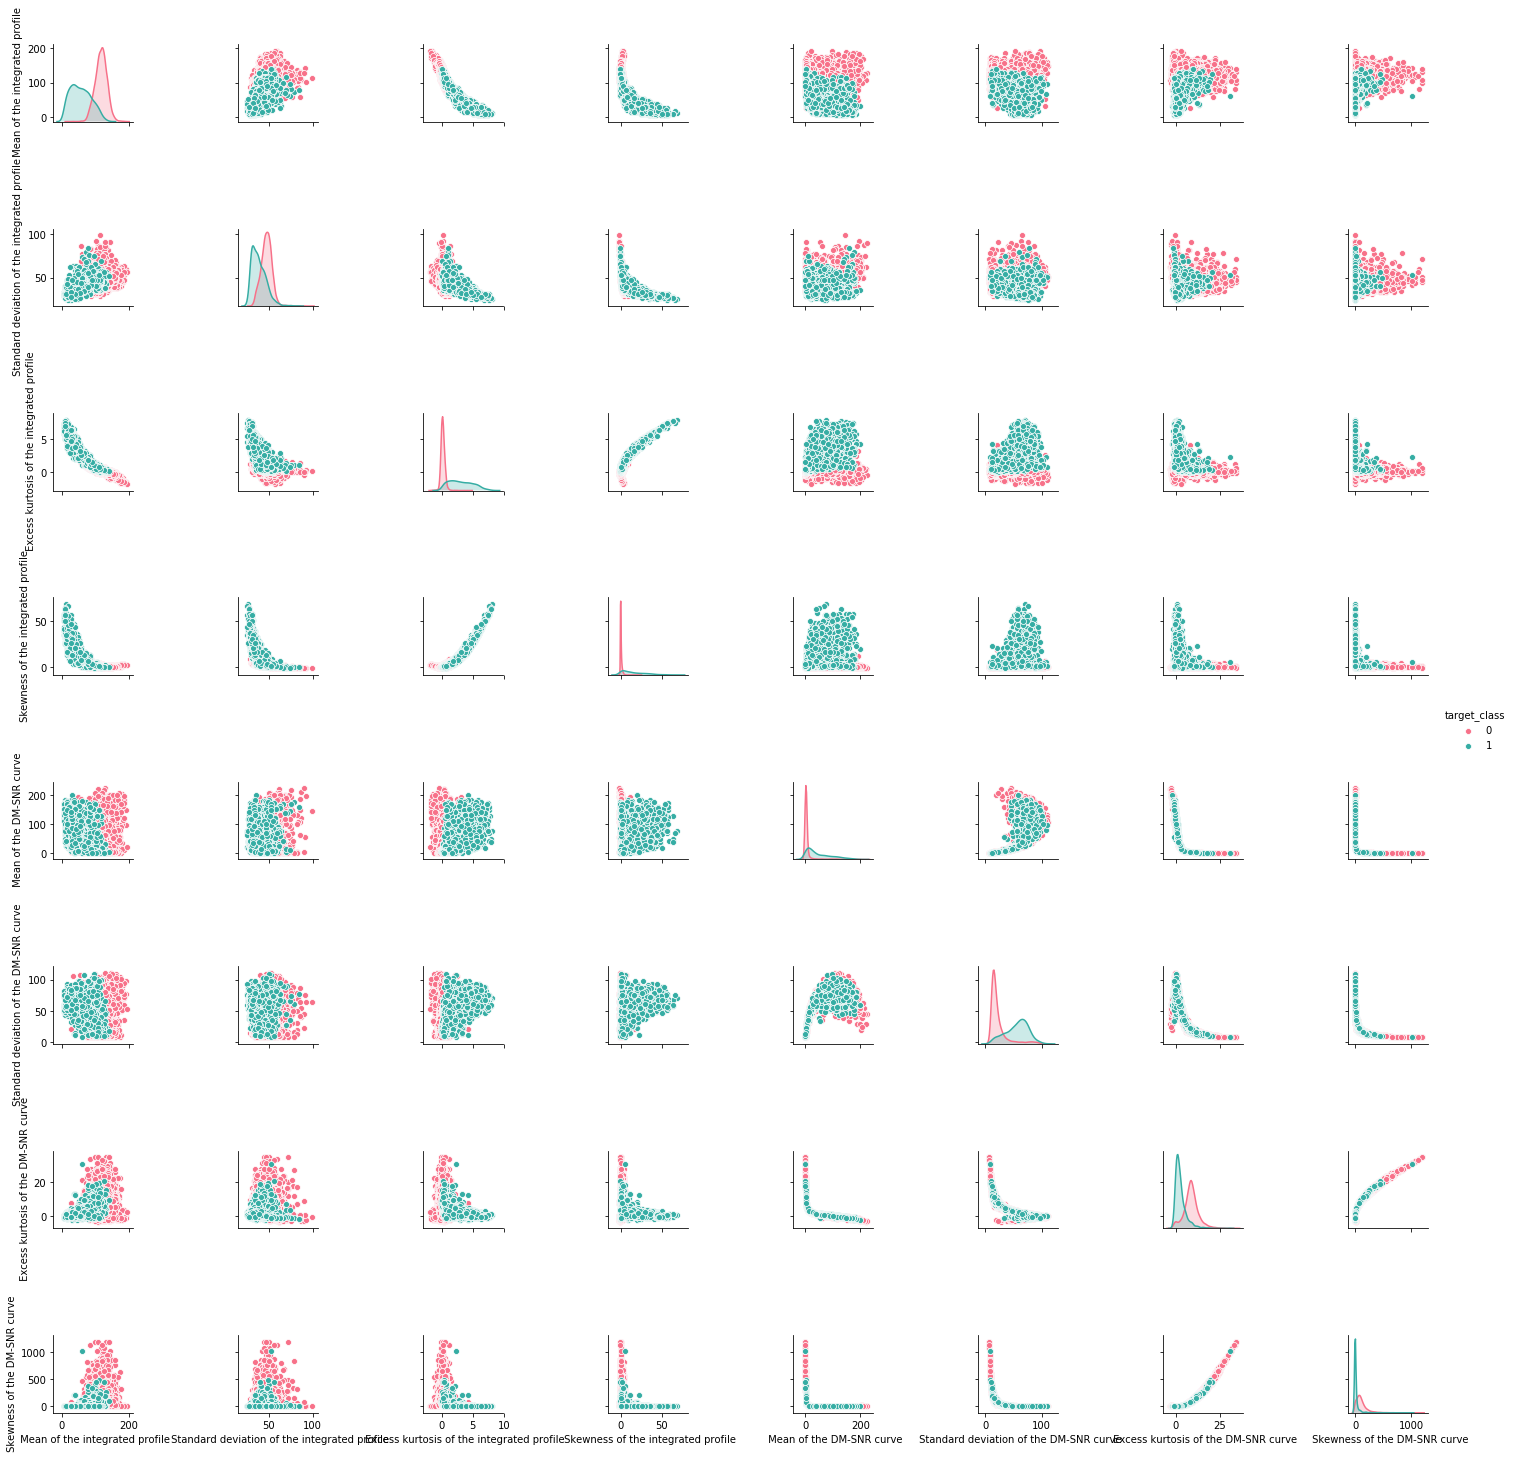
\includegraphics[scale=0.24]{data-correlation.png}
        \newline Kita dapat melihat bahwa data kita cukup dapat dipisahkan pada sebagian besar kolom.
        \newline 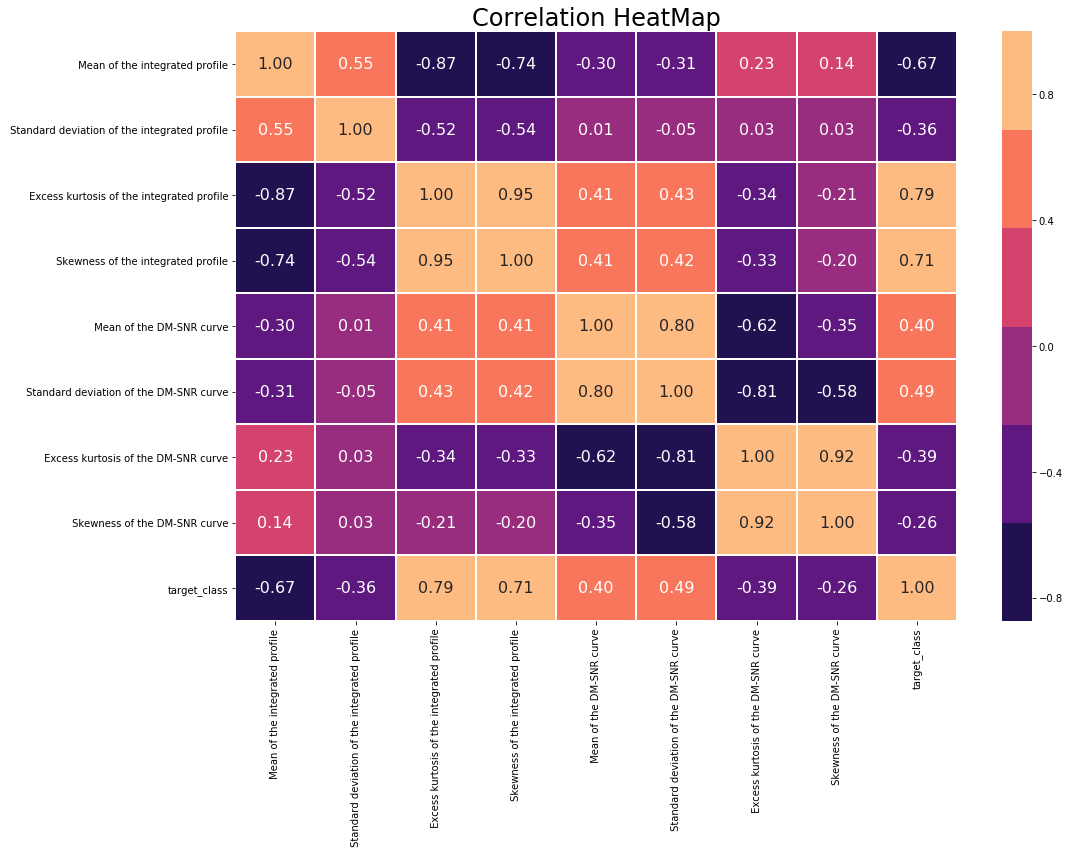
\includegraphics[scale=0.35]{data-correlation-2.png}
        \newline Sebagian besar kolom sudah terkait atau berasal dari satu atau yang lain, dan kita bisa melihatnya dengan jelas pada beberapa sel di atas.
        
        \item Membandingkan Rata-Rata dengan Standar Deviasi
        \begin{enumerate}
        \item Rata-Rata
        \newline 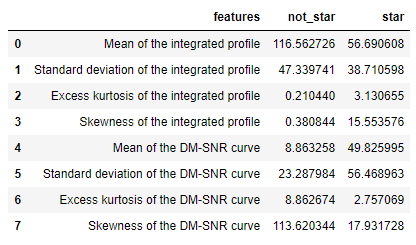
\includegraphics[scale=1]{mean-compare.png}
        \newpage
        \item Standar Deviasi
        \newline 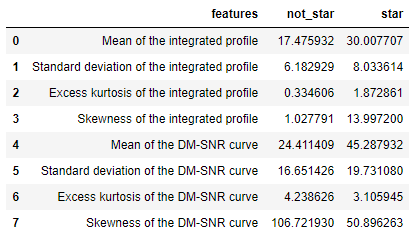
\includegraphics[scale=1]{std-compare.png}
        \end{enumerate}
        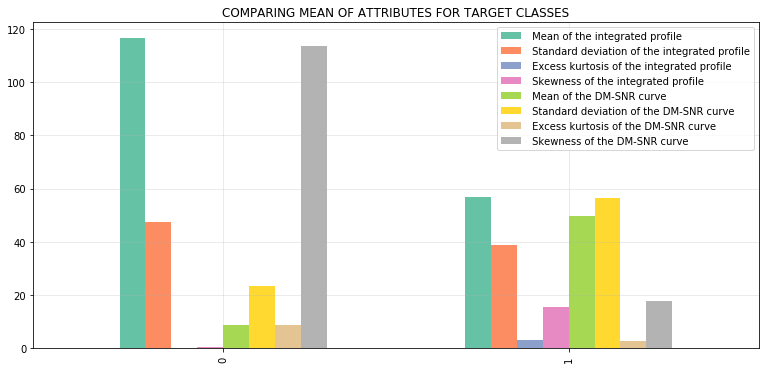
\includegraphics[scale=0.475]{mean-compare-2.png}
        \newline 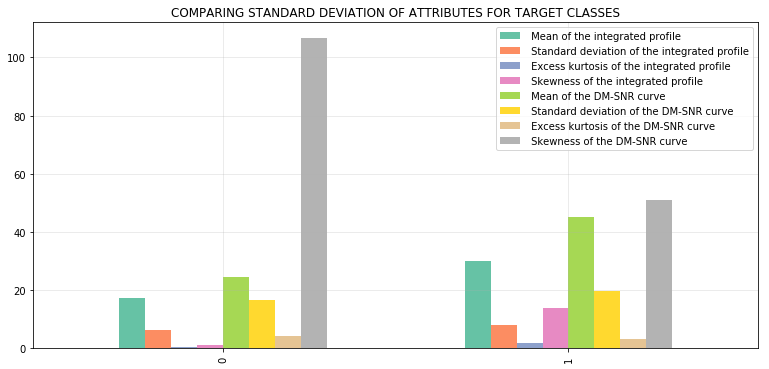
\includegraphics[scale=0.475]{std-compare-2.png}
        \newline 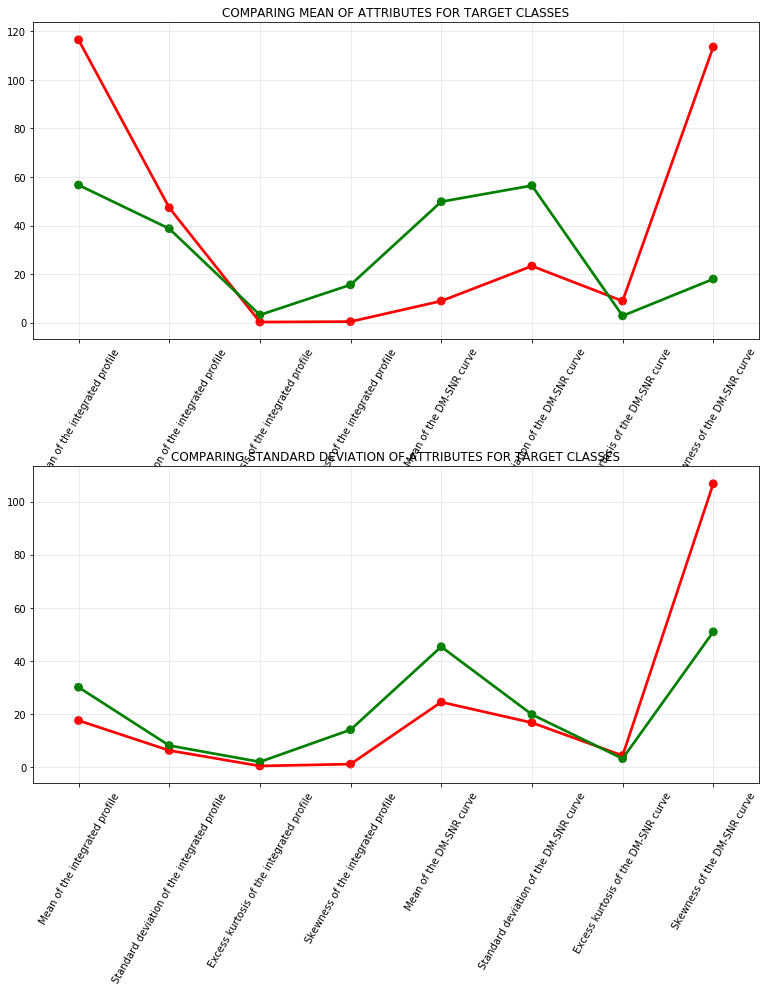
\includegraphics[scale=0.475]{mean-std-compare.png}
        \newline Hijau = Bintang, Merah = Bukan Bintang
        
        \newpage
        
        \item Melihat Distribusi dari variabel
        \newline 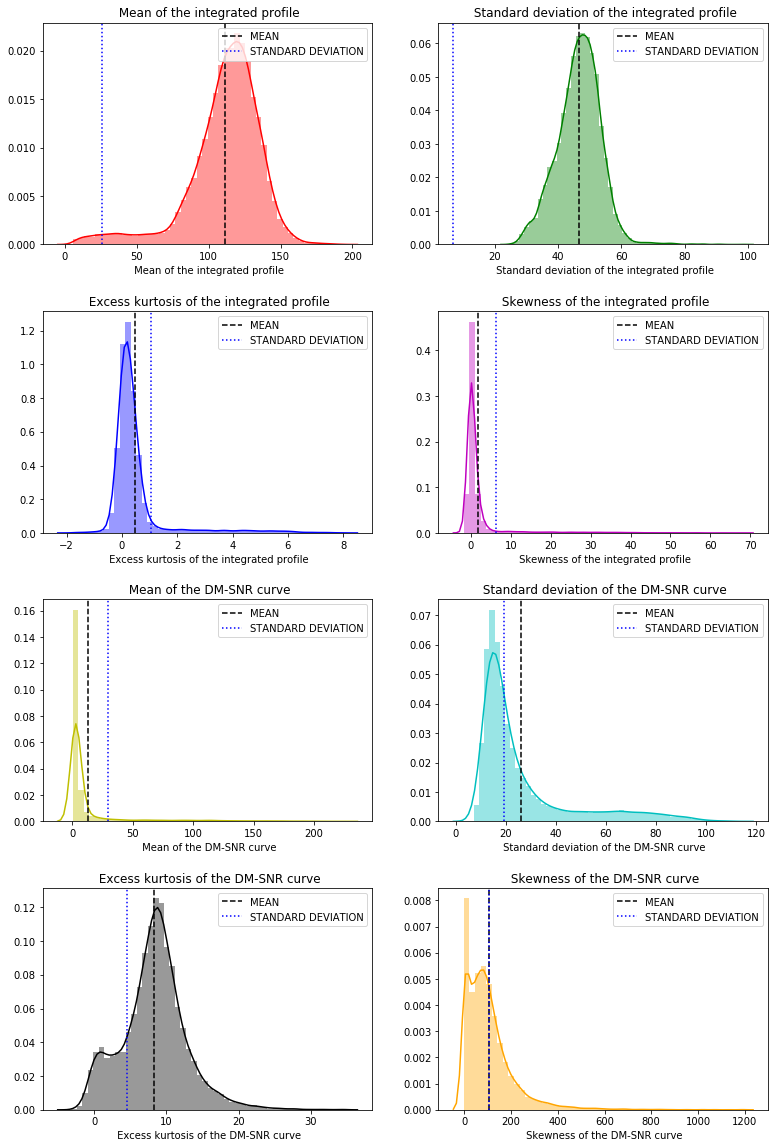
\includegraphics[scale=0.475]{data-distribution.png}
    
    \end{enumerate}
    
    \newpage
    
    \subsection{Data Preprocessing}
    
    \begin{enumerate}
        
        \item Memisahkan Fitur dengan Target
        \newline 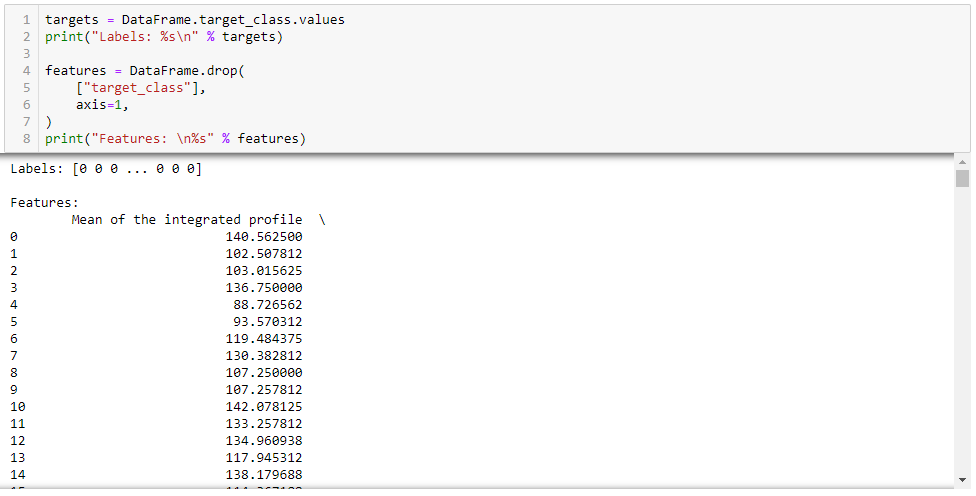
\includegraphics[scale=0.5]{split-target-feature.png}
        
        \item Mengskalasikan Fitur yang ada dengan MinMaxScalar
        \newline 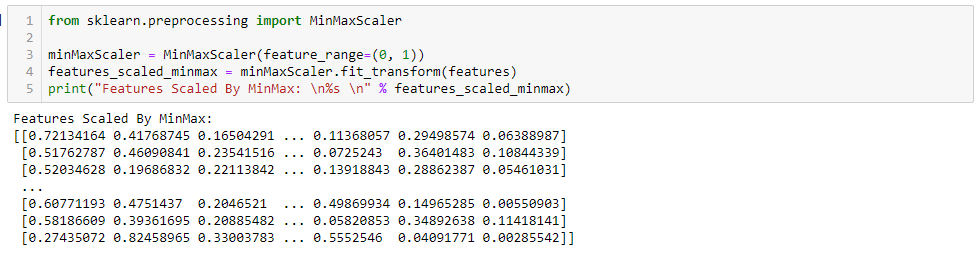
\includegraphics[scale=0.5]{min-max-scalar.png}
        
    \end{enumerate}

 %\texttt{\textbackslash cite\{\ldots\}} command in \texttt{main.tex} \cite{bibtex}. 

\hspace{1 cm}

\newpage

%%%%%%%%%%%%%%%%%%%%%%%%%%%%%%%%%%%%%%%%%%%%%%%%%%%%%%%%%%%%%%%%%%%%%%%%%%%%%%%%%%%%%%%%%

\section{Evaluasi Model}

Sebelum menggunakan model, kita akan mencari parameter yang dapat dianggap terbaik menggunakan GridSearch dari SciKit-Learn.
\newline 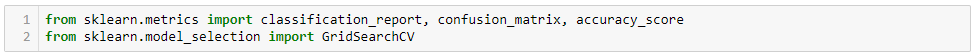
\includegraphics[scale=0.575]{ml-model.png}
\newline

    \subsection{Logistic Regression}
    \newline
    \newline Parameter yang akan dicari adalah: `C`
    \newline 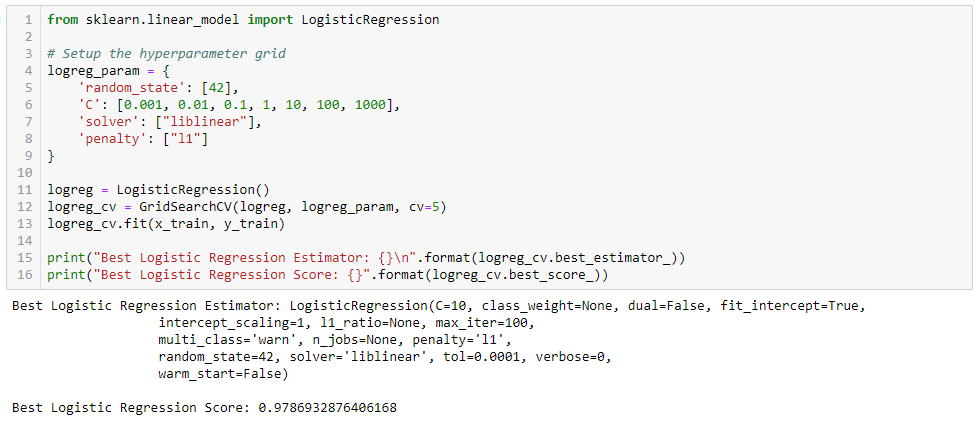
\includegraphics[scale=0.535]{logreg-tune.png}
    \newline
    \newline Setelah didapatkan best parameternya, gunakan ke dalam model.
    \newline 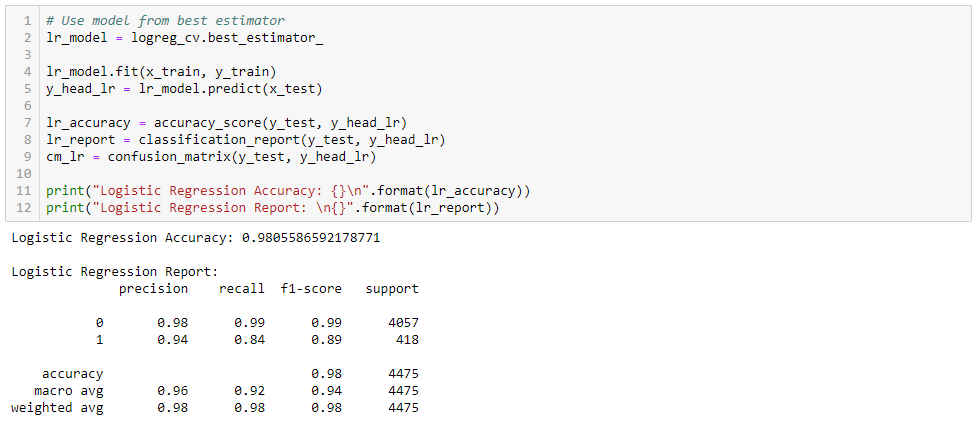
\includegraphics[scale=0.535]{logreg-model.png}
    
    \newpage
    
    \subsection{Decision Tree Classifier}
    \newline
    \newline Parameter yang akan dicari adalah: `max\_depth`
    \newline 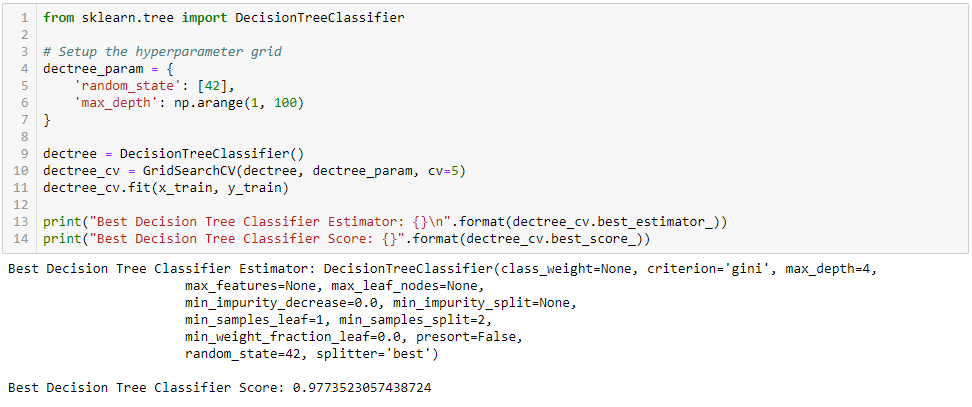
\includegraphics[scale=0.535]{dctree-tune.png}
    \newline
    \newline Setelah didapatkan best parameternya, gunakan ke dalam model.
    \newline 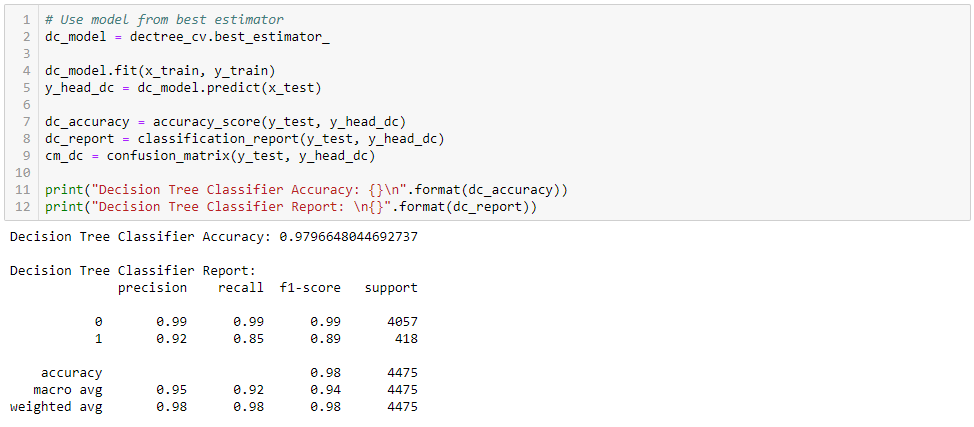
\includegraphics[scale=0.535]{dctree-model.png}
    
    \newpage
    
    \subsection{Random Forest Classifier}
    \newline
    \newline Parameter yang akan dicari adalah: `n\_estimators`
    \newline 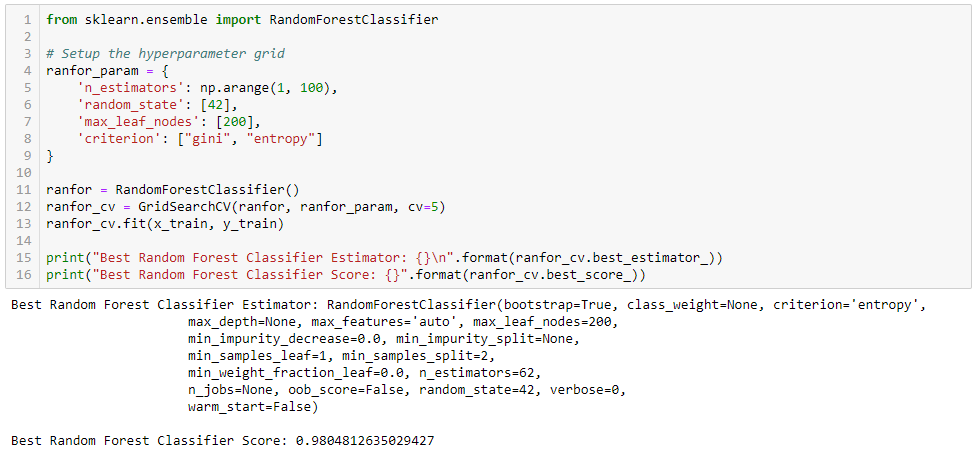
\includegraphics[scale=0.535]{rfc-tune.png}
    \newline
    \newline Setelah didapatkan best parameternya, gunakan ke dalam model.
    \newline 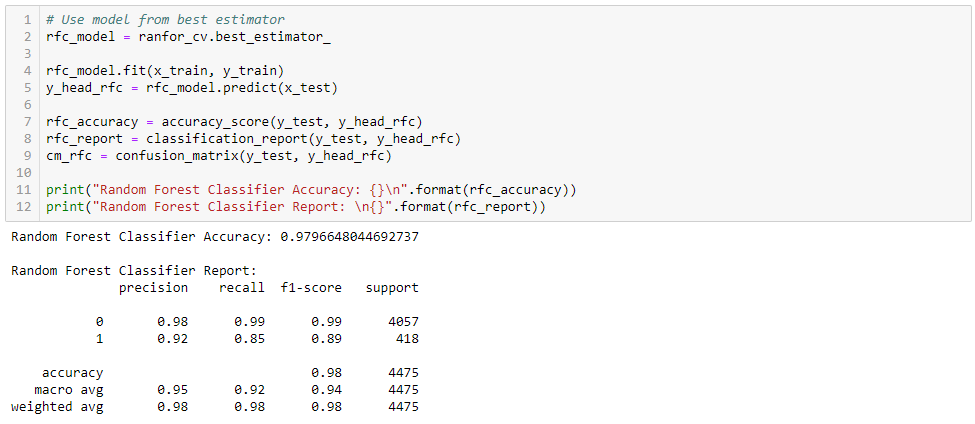
\includegraphics[scale=0.535]{rfc-model.png}
    
    \newpage
    
    \subsection{Naive Bayes Classifier}
    \newline
    \newline Tidak ada parameter yang dapat di tune-up
    \newline 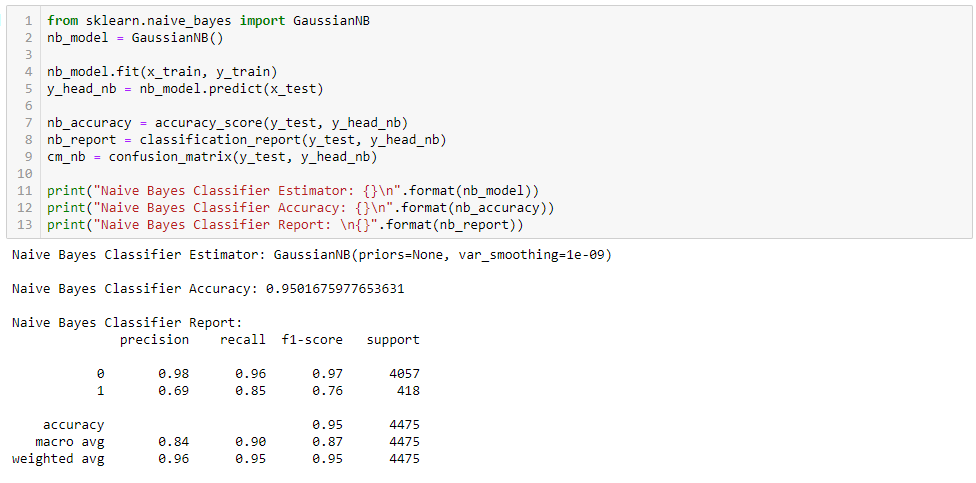
\includegraphics[scale=0.535]{nb-model.png}
    
    \newpage
    
    \subsection{K Nearest Neighbor}
    \newline
    \newline Parameter yang akan dicari adalah: `n\_neighbors', 'weights`
    \newline 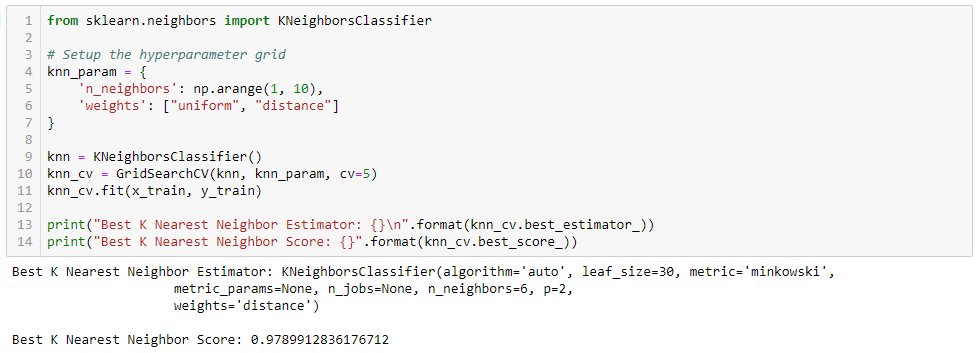
\includegraphics[scale=0.535]{knn-tune.png}
    \newline
    \newline Setelah didapatkan best parameternya, gunakan ke dalam model.
    \newline 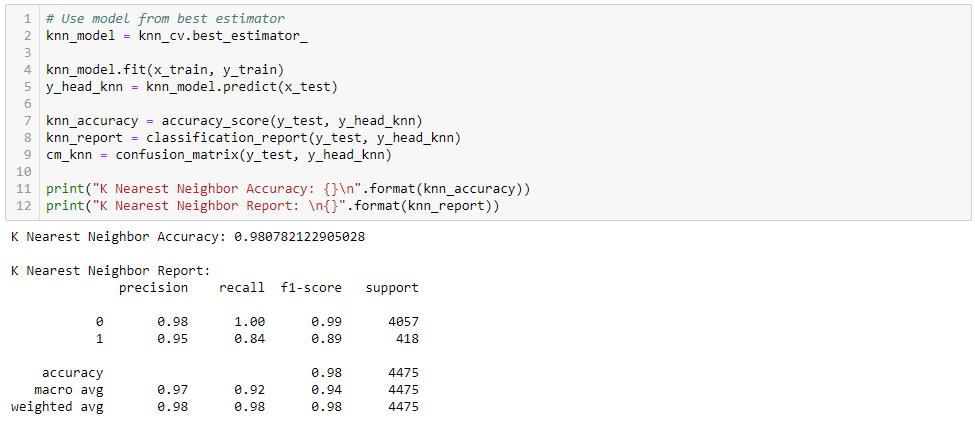
\includegraphics[scale=0.535]{knn-model.png}
    
    \newpage
    
    \subsection{Support Vector Machine}
    \newline
    \newline Parameter yang akan dicari adalah: `C`
    \newline 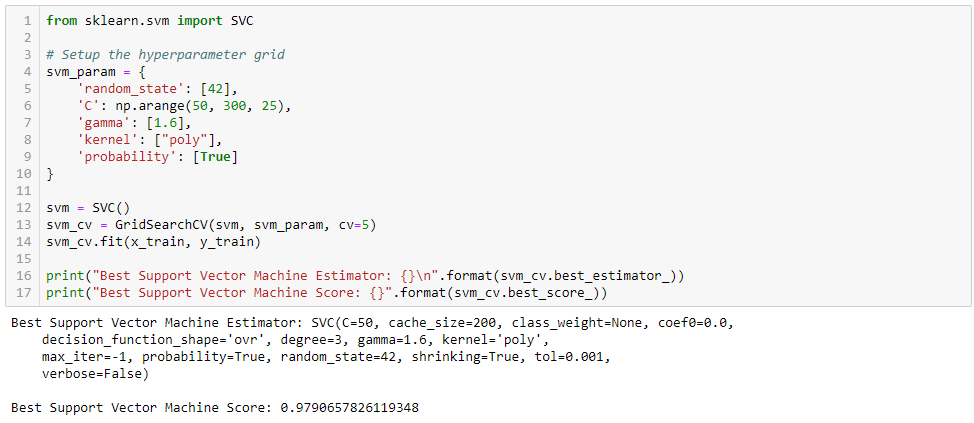
\includegraphics[scale=0.535]{svm-tune.png}
    \newline
    \newline Setelah didapatkan best parameternya, gunakan ke dalam model.
    \newline 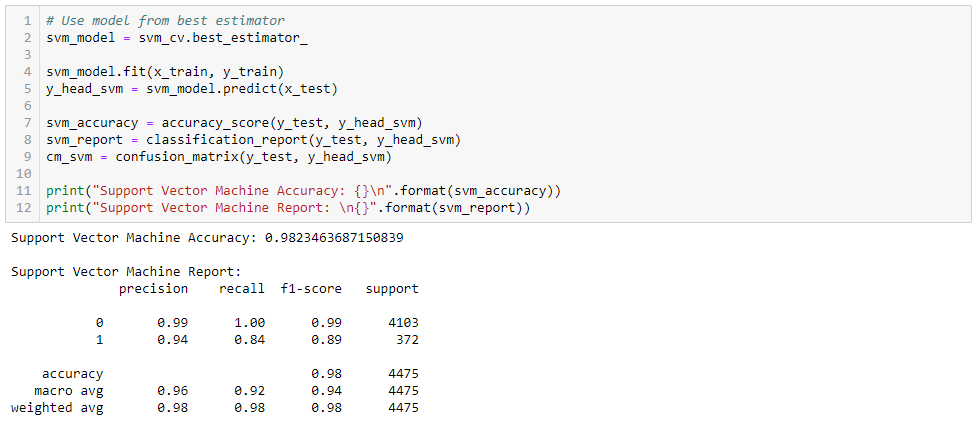
\includegraphics[scale=0.535]{svm-model.png}

 %\texttt{\textbackslash cite\{\ldots\}} command in \texttt{main.tex} \cite{bibtex}. 

\hspace{1 cm}
\newpage

%%%%%%%%%%%%%%%%%%%%%%%%%%%%%%%%%%%%%%%%%%%%%%%%%%%%%%%%%%%%%%%%%%%%%%%%%%%%%%%%%%%%%%%%%

\section{Kesimpulan}

    \subsection{Confusion Matrix}
    \newline 
    \newline 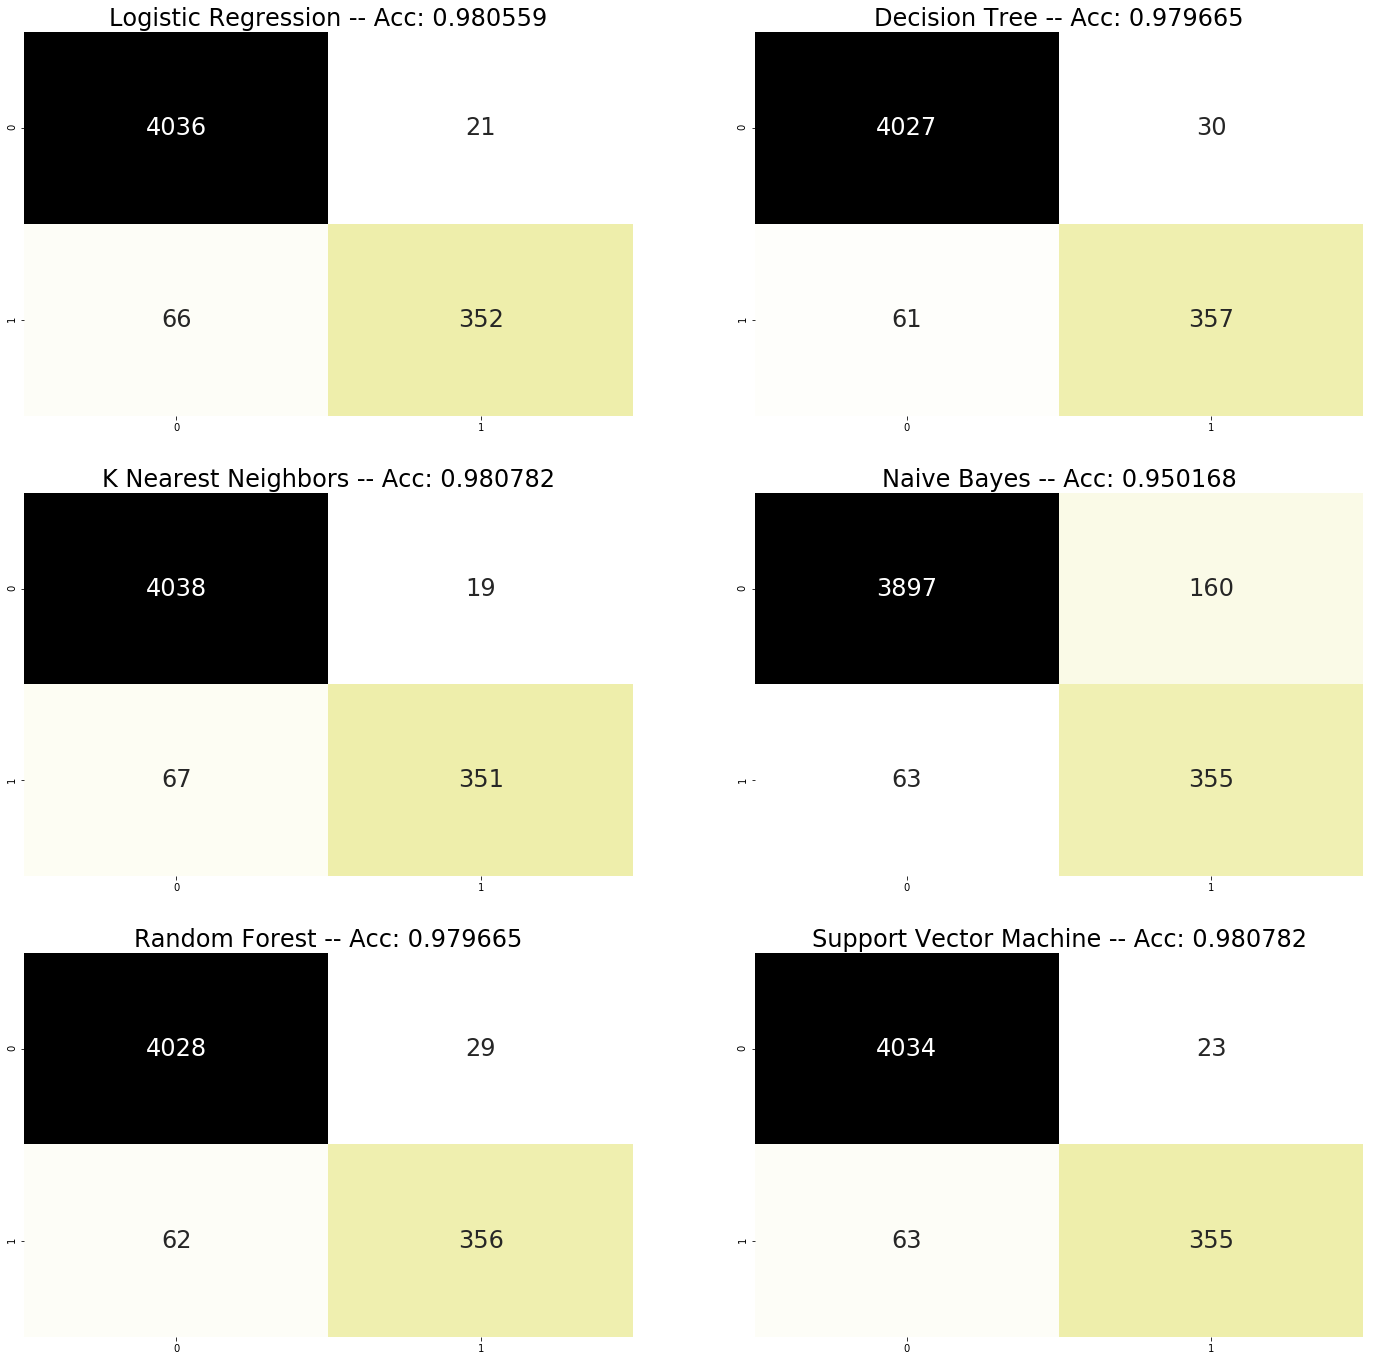
\includegraphics[scale=0.285]{confusion-matrix.png}
    
    \newpage
    
    \subsection{Perbandingan Akurasi}
    \newline 
    \newline 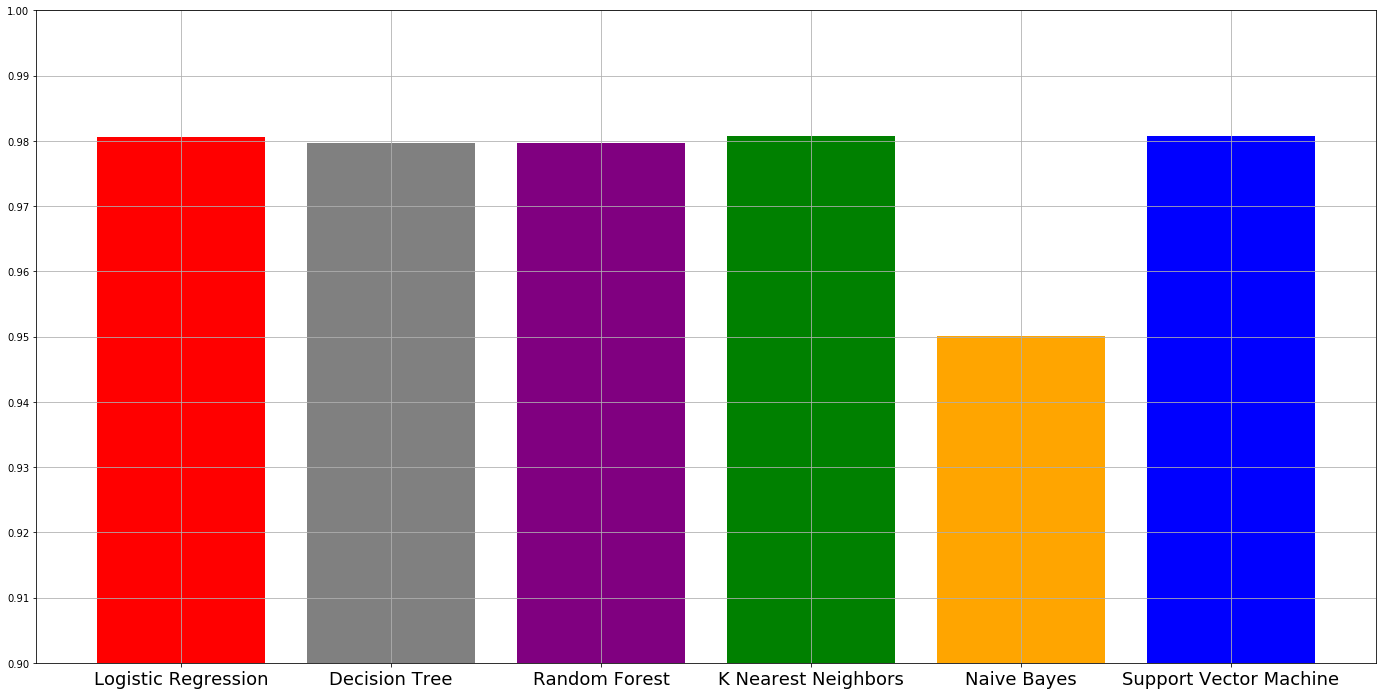
\includegraphics[scale=0.25]{bar-chart-comparison.png}

\subsection{Tingkat Kesalahan Klasifikasi}

\begin{enumerate}

    \item Logistic Regression:
    \newline (21 + 66) / 4475 = 0.0194413407821229
    \newline Sekitar 1.94 \%
    
    \item Decision Tree:
    \newline (30 + 61) / 4475 = 0.0203351955307263
    \newline Sekitar 2.03 \%
    
    \item K Nearest Neighbors:
    \newline (19 + 67) / 4475 = 0.0192178770949721‬
    \newline Sekitar 1.92 \%
    
    \item Naive Bayes:
    \newline (160 + 63) / 4475 = 0.0498324022346369‬‬
    \newline Sekitar 4.98 \%
    
    \item Random Forest:
    \newline (29 + 62) / 4475 = 0.0203351955307263‬‬‬
    \newline Sekitar 2.03 \%
    
    \item Support Vector Machine:
    \newline (23 + 63) / 4475 = 0.0192178770949721‬‬‬
    \newline Sekitar 1.92 \%
    
\end{enumerate}

 %\texttt{\textbackslash cite\{\ldots\}} command in \texttt{main.tex} \cite{bibtex}. 

\hspace{1 cm}
\newpage

%%%%%%%%%%%%%%%%%%%%%%%%%%%%%%%%%%%%%%%%%%%%%%%%%%%%%%%%%%%%%%%%%%%%%%%%%%%%%%%%%%%%%%%%%

\section{Kontribusi Anggota}

Project dibuat dengan membutuhkan waktu sekitar 12 jam kerja, memakan waktu kurang lebih 4-5 jam untuk mencari referensi, 5-6 jam untuk mengeksekusi coding dan paling banyak memakan waktu yaitu pada saat mencari parameter dengan GridSearch, 2-3 jam untuk membuat laporan.

\begin{enumerate}

    \item Steven - 000.000.13433
    \newline Exploratory Data Analysis, Modelling
    
    \item Basilius Bias Astho Christyono - 000.000.13536
    \newline Exploratory Data Analysis, Modelling, Menyusun Laporan
    
    \item Raynaldi - 000.000.13654
    \newline Exploratory Data Analysis, Menyusun Laporan
    
\end{enumerate}

 %\texttt{\textbackslash cite\{\ldots\}} command in \texttt{main.tex} \cite{bibtex}. 

\hspace{1 cm}
\newpage

\bibliographystyle{plain}
\bibliography{biblist}

\end{document}